% Adapted from J. Leon, https://tex.stackexchange.com/questions/432312/how-do-i-draw-an-lstm-cell-in-tikz
\usetikzlibrary{positioning, fit, arrows.meta, shapes}

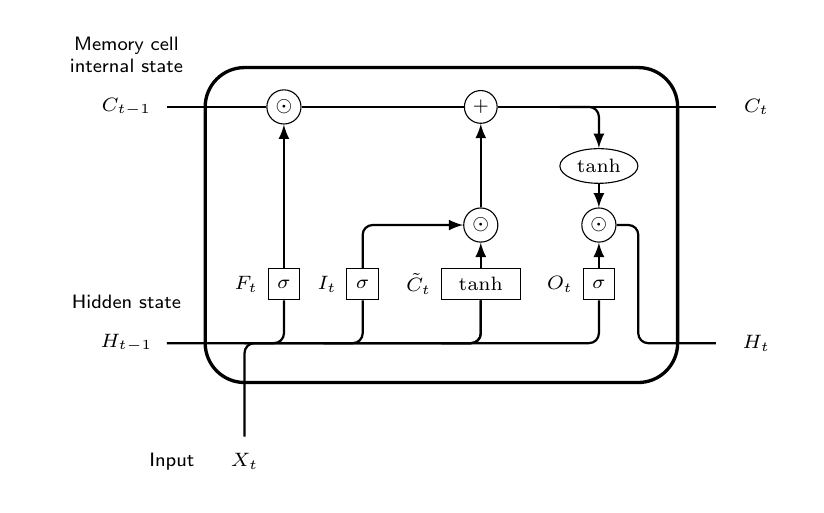
\begin{tikzpicture}[
    font=\sf \scriptsize,
    >=latex,
    % Styles
    cell/.style={
        rectangle,
        rounded corners=5mm,
        draw,
        very thick,
        },
    operator/.style={
        circle,
        draw,
        inner sep=1.5pt,
        minimum height =0.4cm,
        },
    function/.style={
        ellipse,
        draw,
        inner sep=2pt
        },
    ct/.style={
        line width = .75pt,
        minimum height=0.60cm,
        minimum width=1cm,
        inner sep=2pt,
        },
    gt/.style={
        rectangle,
        draw,
        minimum width=0.4cm,
        minimum height=0.4cm,
        inner sep=2pt
        },
    inoutlabels/.style={
        text width=2cm,
        align=center,
        },
    Arrow/.style={
        rounded corners=.125cm,
        thick,
        },
    ]

    \node [cell, minimum height =4cm, minimum width=6cm] at (0,0){} ;

    \node [gt, label={left:$\boldsymbol{F}_{t}$}] (ibox1) at (-2,-0.75) {$\sigma$};
    \node [gt, label={left:$\boldsymbol{I}_{t}$}] (ibox2) at (-1,-0.75) {$\sigma$};
    \node [gt, minimum width=1cm, label={left:$\boldsymbol{\tilde{C}}_{t}$}] (ibox3) at (0.5,-0.75) {$\tanh$};
    \node [gt, label={left:$\boldsymbol{O}_{t}$}] (ibox4) at (2,-0.75) {$\sigma$};

    \node [operator] (mux1) at (-2,1.5) {$\odot$};
    \node [operator] (add1) at (0.5,1.5) {+};
    \node [operator] (mux2) at (0.5,0) {$\odot$};
    \node [operator] (mux3) at (2,0) {$\odot$};
    \node [function] (func1) at (2,0.75) {$\tanh$};

    \node[ct, label={[inoutlabels]Memory cell internal state}] (c) at (-4,1.5) {$\boldsymbol{C}_{t-1}$};
    \node[ct, label={[inoutlabels]Hidden state}] (h) at (-4,-1.5) {$\boldsymbol{H}_{t-1}$};
    \node[ct, label={[inoutlabels, align=right]left:Input}] (x) at (-2.5,-3) {$\boldsymbol{X}_{t}$};

    \node[ct] (c2) at (4,1.5) {$\boldsymbol{C}_{t}$};
    \node[ct] (h2) at (4,-1.5) {$\boldsymbol{H}_{t}$};

    \draw [Arrow] (c) -- (mux1) -- (add1) -- (c2);

    \draw [Arrow] (h) -| (ibox4);
    \draw [Arrow] (h -| ibox1)++(-0.5,0) -| (ibox1);
    \draw [Arrow] (h -| ibox2)++(-0.5,0) -| (ibox2);
    \draw [Arrow] (h -| ibox3)++(-0.5,0) -| (ibox3);
    \draw [Arrow] (x) -- (x |- h)-| (ibox3);

    \draw [->, Arrow] (ibox1) -- (mux1);
    \draw [->, Arrow] (ibox2) |- (mux2);
    \draw [->, Arrow] (ibox3) -- (mux2);
    \draw [->, Arrow] (ibox4) -- (mux3);
    \draw [->, Arrow] (mux2) -- (add1);
    \draw [->, Arrow] (add1 -| func1)++(-0.5,0) -| (func1);
    \draw [->, Arrow] (func1) -- (mux3);

    \draw [-, Arrow] (mux3 |- h2)++(0.5,0.5) |- (h2);
    \draw [-, Arrow] (mux3 |- h2)++(0.5,0.5) |- (mux3);
\end{tikzpicture}
